\documentclass[conference]{IEEEtran}

\usepackage[utf8]{inputenc}
\usepackage[english]{babel}
\usepackage{graphicx}
\usepackage{tikz}
\usetikzlibrary{positioning,arrows.meta}

\begin{document}

\title{Implementing 'Gordon': A NAO Robot Receptionist to Enhance Efficiency in Critical Services Using Choregraphe and Python}

\author{
\IEEEauthorblockN{
        Diana Milligan\IEEEauthorrefmark{1},
        Filip Hanuš\IEEEauthorrefmark{1},
        Harry Williams\IEEEauthorrefmark{1},\\
        Jack Thompson\IEEEauthorrefmark{1},
        Natalie Leung\IEEEauthorrefmark{1}
}
\IEEEauthorblockA{
        \IEEEauthorrefmark{1}School of Engineering, College of Art, Technology and Environment,\\ University of the West of England, Bristol, UK\\
        Email: diana2.milligan, filip2.hanus, harry4.williams, jack2.ould, wing7.leung\}@live.uwe.ac.uk}
}

\maketitle

\begin{abstract}

This paper presents what is in this abstract. 

\end{abstract}

\begin{IEEEkeywords}

NAO Robot, Human Robot Interaction.

\end{IEEEkeywords}

\section{Distribution of Work} This project has been equally distributed to and completed by the authors of this report.

\section{Introduction}

The purpose of this project is to use a Nao robotic platform to effectively perform a task that requires direct interaction with human. 
There are many different metrics that can be used to quantify the success of such a system, but as a broader definition an effective system 
should be able to receive and convey relevant information to an untrained user to achieve a wider goal.

A task that lends itself to this project brief is a reception environment, particularly in a medical setting. According to 
Mallorie \cite{mallorie2024}, managerial staff shortages within the NHS has pushed clinical staff to spend more time on administrative task over 
patient-facing care. To effectively reduce staffing requirements and thus make the running of medical centres less resource intensive, robotic 
systems can be integrated to alleviate the bulk of repetitive tasks. A good low-risk opportunity for this kind of integration is within a 
receptionist role where any possible errors are of a significantly lower severity than other roles (e.g. medical diagnosis and treatment).
A study conducted by Sutherland et al. \cite{Sutherland2019} tested the concept of a robotic receptionist for medical purposes, concluding that the robot displayed a 
"professional level of friendliness" that made it suited the role. However, the testing used a Wizard-of-Oz method with the robot only 
used as the interface between a user and a remote operator. Had all the behaviours been generated by the robot, there could have been 
a significant difference in how it was perceived by users.

Methods to create a sense of authority for robots has been explored through many different ways, many of which can be implemented within 
this project. Rae et al. \cite{Rae2013} explored the effect of height on robotic telepresence systems, concluding that a shorter "leader" was less persuasive 
for a the human follower. As well as the robot's stature, Rossi (need citation) found that contextual information such as the location of an interaction 
helped users infer the robot’s role.

Appearance has been argued to be a less important factor by Natarajan and Gombolay (need citation) who tested a variety of different variables for artificial agents, with 
behaviour being " the most significant factors in predicting the trust and compliance with the robot" rather 
than physical appearance. A Nao platform has been used by Cormier et al. \cite{cormier2013} to test the limitations of such compliance, finding that users would 
refuse to follow challenging orders from a robot if factors such as perceived intelligence or professionalism were compromised.

\section{Scope and Assumptions} In Scope:
\begin{itemize}
        \item Initiate client/robot interaction with a waving motion
        \item Greet client and identify the staff member they have an appointment with
        \item Nao locates the appointment and emails staff that the client has arrived
        \item Create gestures that Nao performs during client/robot interaction    
\end{itemize}

Out of Scope:
\begin{itemize}
        \item Exploring alternative robots
        \item System is not connected to a database of appointments 
\end{itemize}

Assumptions:
\begin{itemize}
        \item Interactions will converse in British English only.
        \item Nao will be positioned out of reach from client users
        \item Nao will always be powered on
\end{itemize}

\section{Technical Implementation}

\subsection{State Machine Description}

\subsubsection{System Start}
\paragraph{Entry Condition:}
\mbox{}\\
The robot/system is powered on or reset. This is the initial state.

\paragraph{Actions:}
\begin{itemize}
  \item Immediately triggers \textbf{Face Detection}, looking for any faces in view.
  \item Checks whether the \emph{number of faces} has changed (i.e., a new face appears).
  \item If a new face is detected, the system attempts to \emph{Learn face (employee)}. If learning is successful, it proceeds with a \emph{Success message}; if unsuccessful, it gives a \emph{Failure message}.
\end{itemize}

\paragraph{Transitions:}
\begin{itemize}
  \item Both the \emph{success} and \emph{failure} learning branches eventually converge and transition to \textbf{State 0}. This is in order to prevent getting stuck due to NAO's technical problems.
\end{itemize}

\begin{figure}
    \centering
    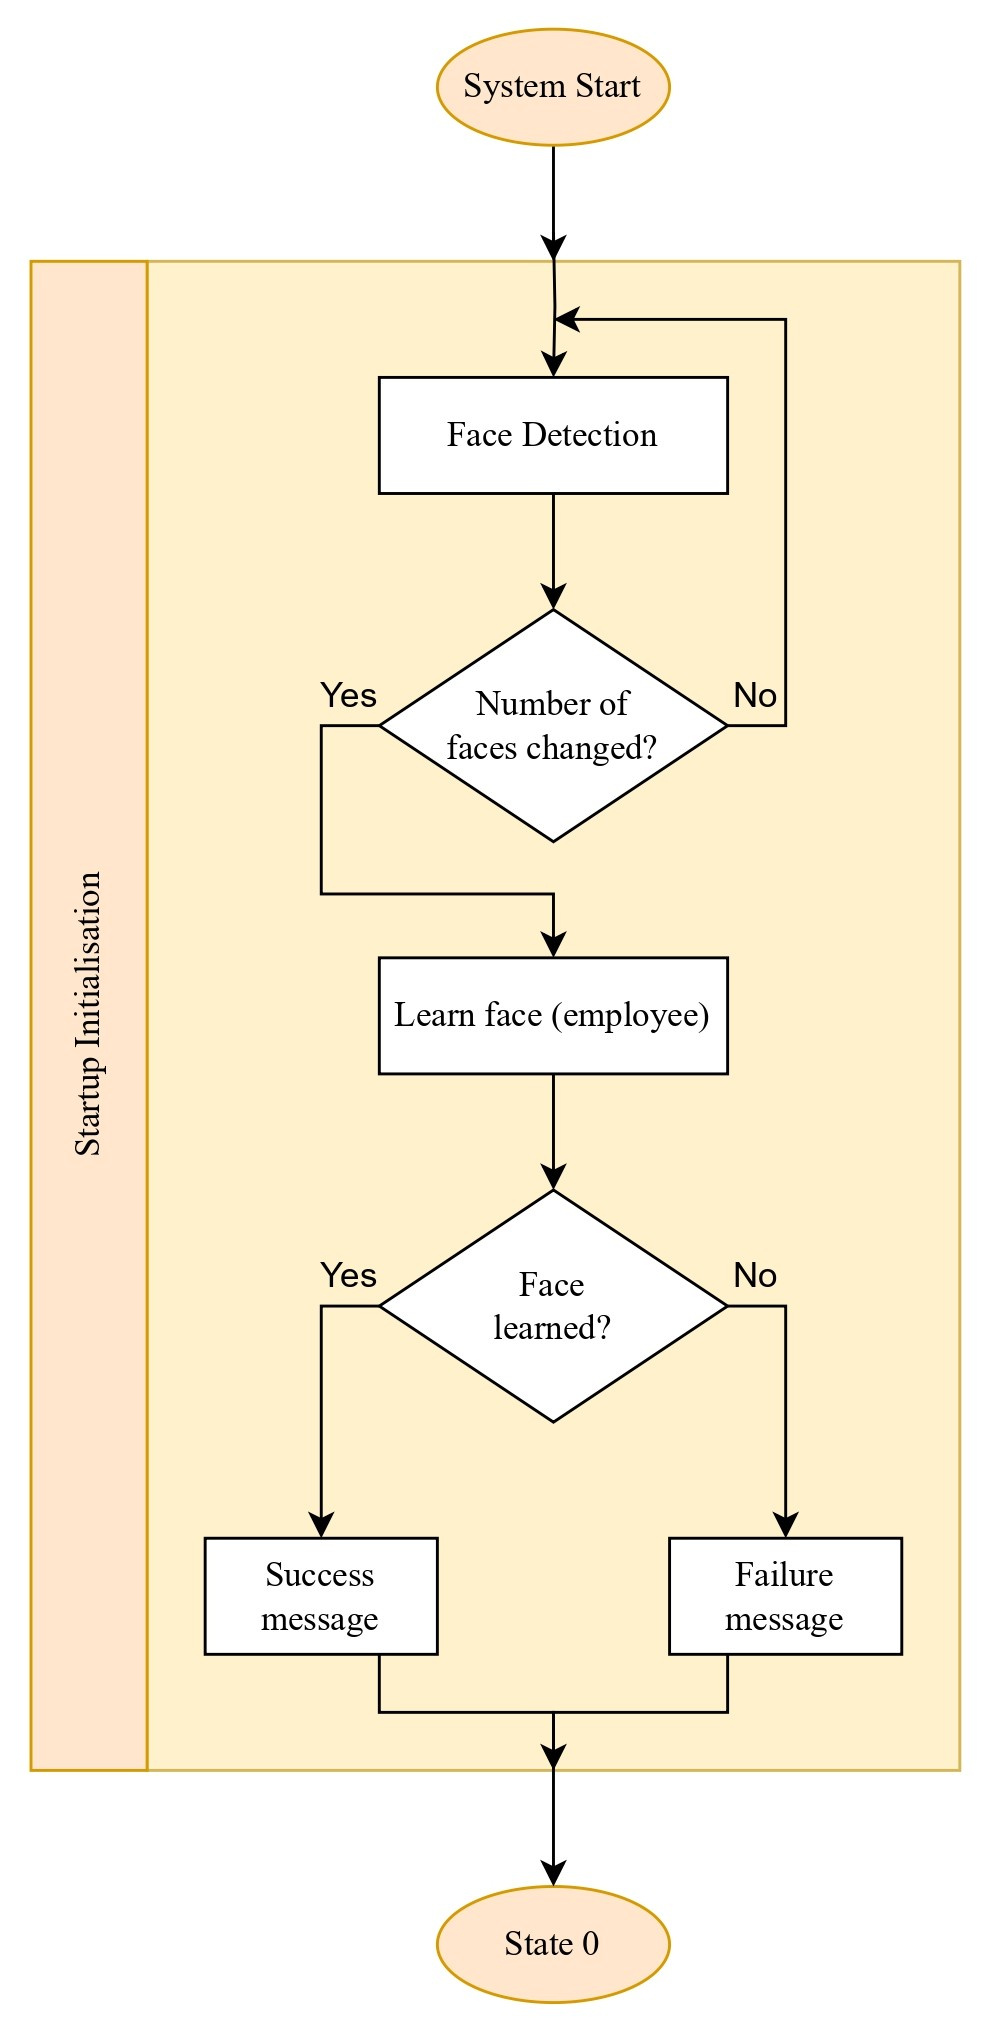
\includegraphics[width=.6\linewidth]{Startup Initialisation.jpg}
    \caption{Startup Initialisation}
    \label{Startup Initialisation}
\end{figure}

\subsubsection{State 0}
\paragraph{Entry Condition:}
\mbox{}\\
The machine enters this state after finishing the initial face-detection/learning process.

\paragraph{Actions:}
\begin{itemize}
  \item Continuously \emph{reads webcam input}.
  \item Monitors for a \emph{wave} via MediaPipe.
\end{itemize}

\paragraph{Transitions:}
\begin{itemize}
  \item If a wave is detected, perform \emph{Action: Wave back} and move to \textbf{State 1}.
  \item If no wave is detected, remain in \textbf{State 0} and continue monitoring.
\end{itemize}

\begin{figure}
    \centering
    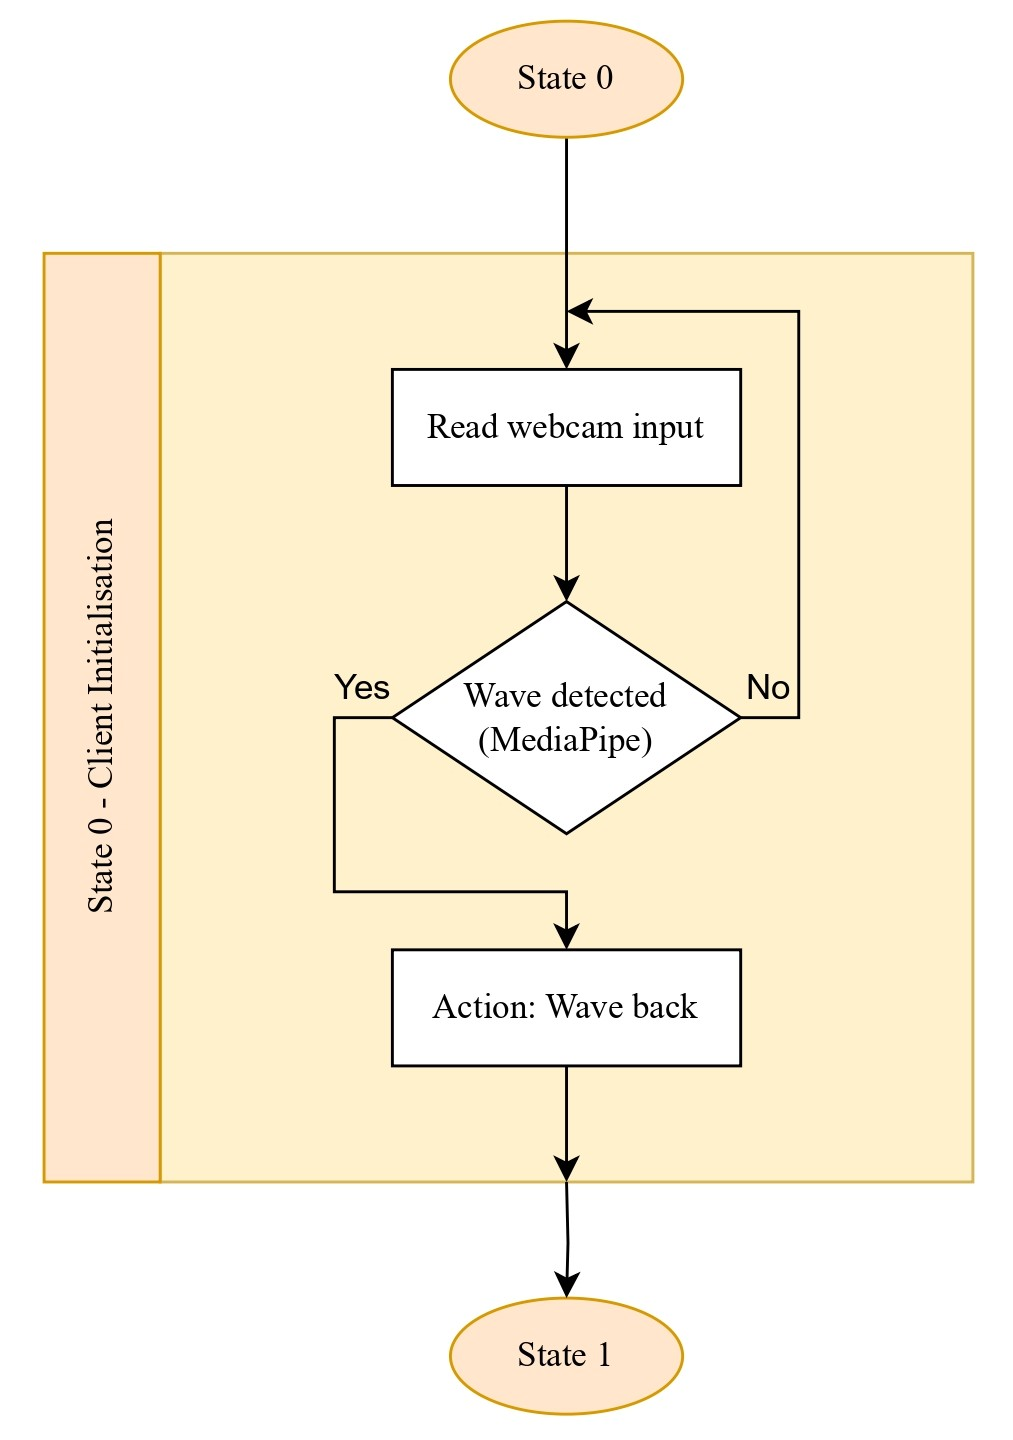
\includegraphics[width=.6\linewidth]{State 0 - Client Initialisation.jpg}
    \caption{State 0 - Client Initialisation}
    \label{State 0 - Client Initialisation}
\end{figure}

\subsubsection{State 1}
\paragraph{Entry Condition:}
\mbox{}\\
A wave has been detected in \textbf{State 0}, triggering the move here (``Client Appointment Initialisation'').

\paragraph{Actions:}
\begin{itemize}
  \item Asks the user if they have an appointment.
  \item Performs \emph{Speech Recognition} to capture their answer.
  \item Checks if the answer is ``yes'' or ``no''.
\end{itemize}

\paragraph{Transitions:}
\begin{itemize}
  \item If \emph{yes}, transition to \textbf{State 2} (handle appointment details).
  \item If \emph{no}, transition to \textbf{State 3} (offer human assistance).
\end{itemize}

\begin{figure}
    \centering
    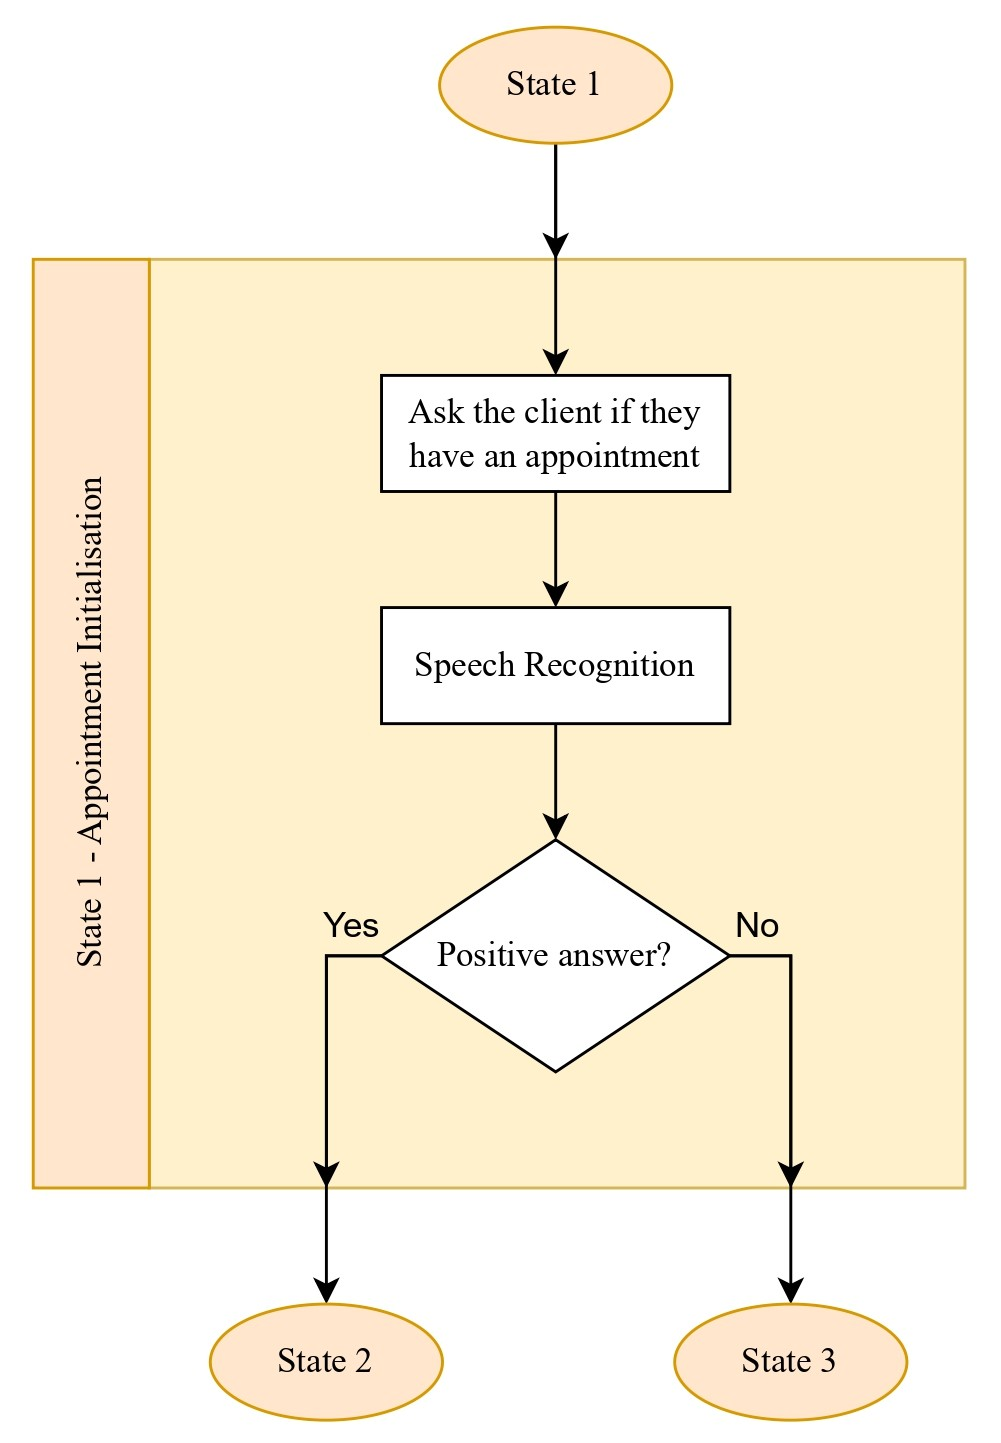
\includegraphics[width=.6\linewidth]{State 1 - Appointment Initialisation.jpg}
    \caption{State 1 - Appointment Initialisation}
    \label{State 1 - Appointment Initialisation}
\end{figure}

\subsubsection{State 2}
\paragraph{Entry Condition:}
\mbox{}\\
User has indicated they do have an appointment.

\paragraph{Actions:}
\begin{itemize}
  \item Prompts for the name of the staff member or the confirmation number.
  \item Uses \emph{Speech Recognition}, then checks if the provided information is found in the database.
  \item Keeps track of the number of failed attempts.
\end{itemize}

\paragraph{Transitions:}
\begin{itemize}
  \item If the name or confirmation number is valid, \emph{nod head} and transition to \textbf{State 4} (staff notification).
  \item If it is invalid, increment the failure count. If failures exceed 2, \emph{shake head} and move to \textbf{State 3}.
\end{itemize}

\begin{figure}
    \centering
    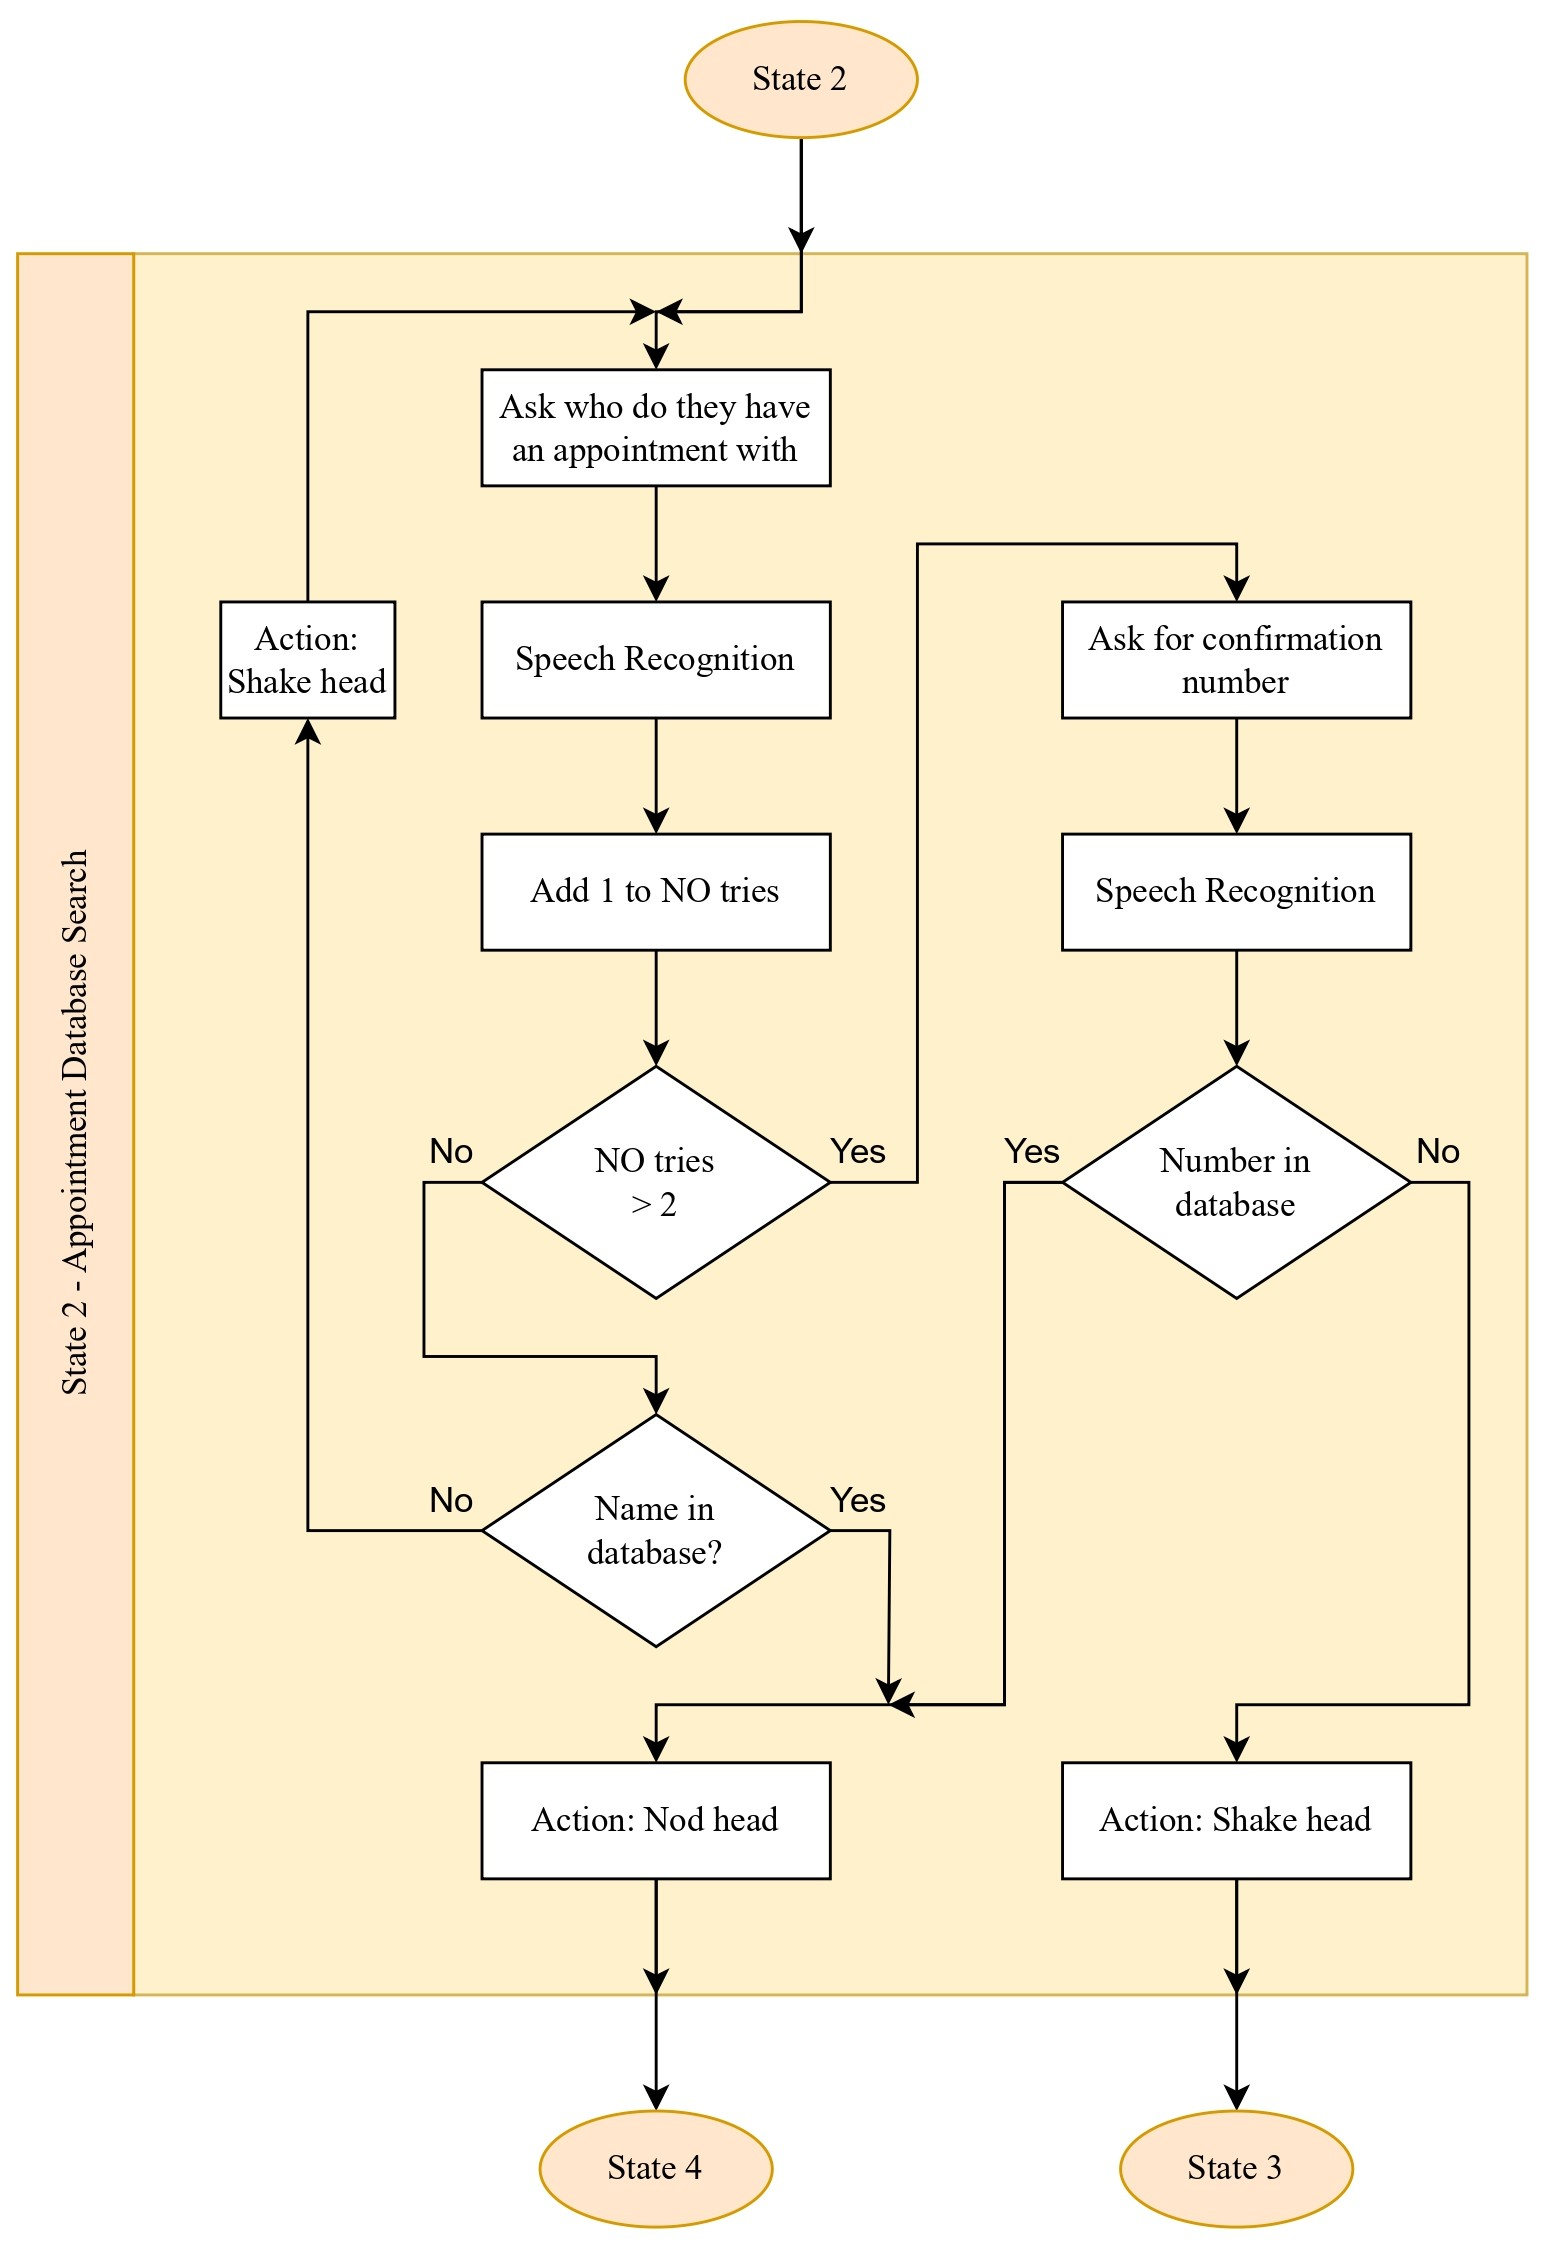
\includegraphics[width=.6\linewidth]{State 2 - Appointment Database Search.jpg}
    \caption{State 2 - Appointment Database Search}
    \label{State 2 - Appointment Database Search}
\end{figure}

\subsubsection{State 3}
\paragraph{Entry Condition:}
\mbox{}\\
Either the user said they have no appointment (from State 1) or they exceeded failures in State 2.

\paragraph{Actions:}
\begin{itemize}
  \item Asks the user if they would like to call a human staff member.
  \item Performs \emph{Speech Recognition} and checks if the answer is positive or negative.
\end{itemize}

\paragraph{Transitions:}
\begin{itemize}
  \item If \emph{yes}, \emph{nod head} and proceed to \textbf{State 4}.
  \item If \emph{no}, \emph{shake head} and return to \textbf{State 0}.
\end{itemize}

\begin{figure}
    \centering
    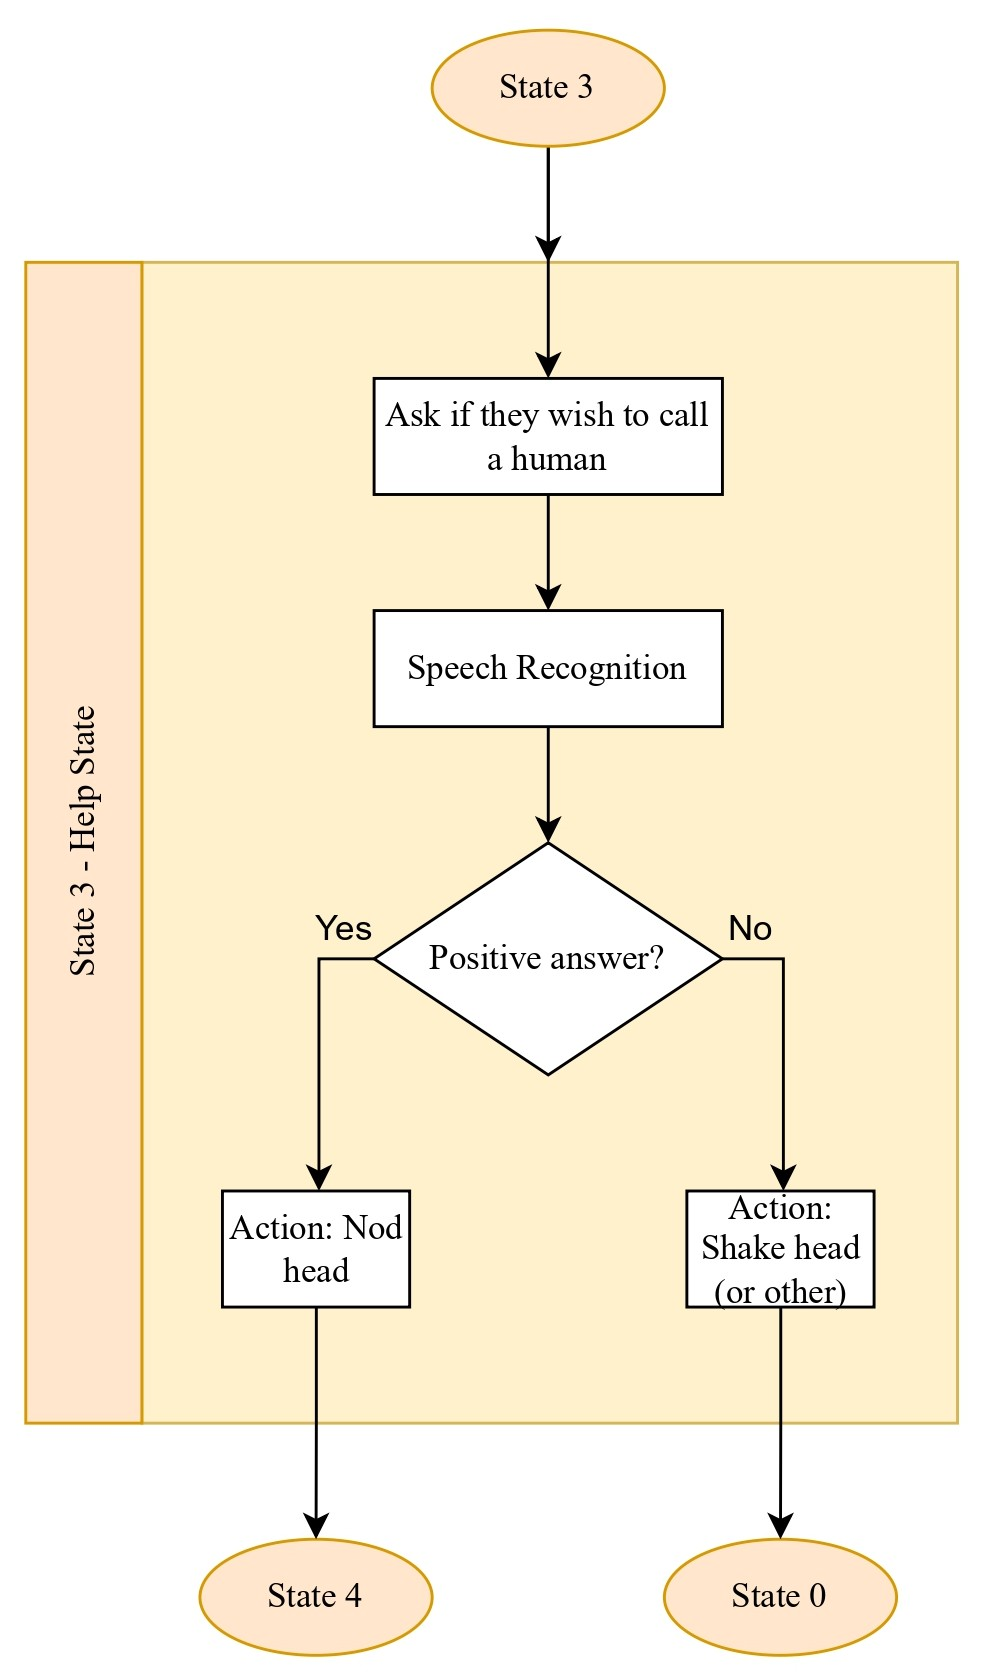
\includegraphics[width=.6\linewidth]{State 3 - Help State.jpg}
    \caption{State 3 - Help State}
    \label{State 3 - Help State}
\end{figure}

\subsubsection{State 4}
\paragraph{Entry Condition:}
\mbox{}\\
Indicates the system must notify staff (arrived from State 2 or State 3).

\paragraph{Actions:}
\begin{itemize}
  \item Performs \emph{Action: Computer Glance}, then sends an email to the specified staff member.
  \item Announces that staff has been notified.
\end{itemize}

\paragraph{Transitions:}
\begin{itemize}
  \item Moves on to \textbf{State 5} after notifying staff and confirming the message was sent.
\end{itemize}

\begin{figure}
    \centering
    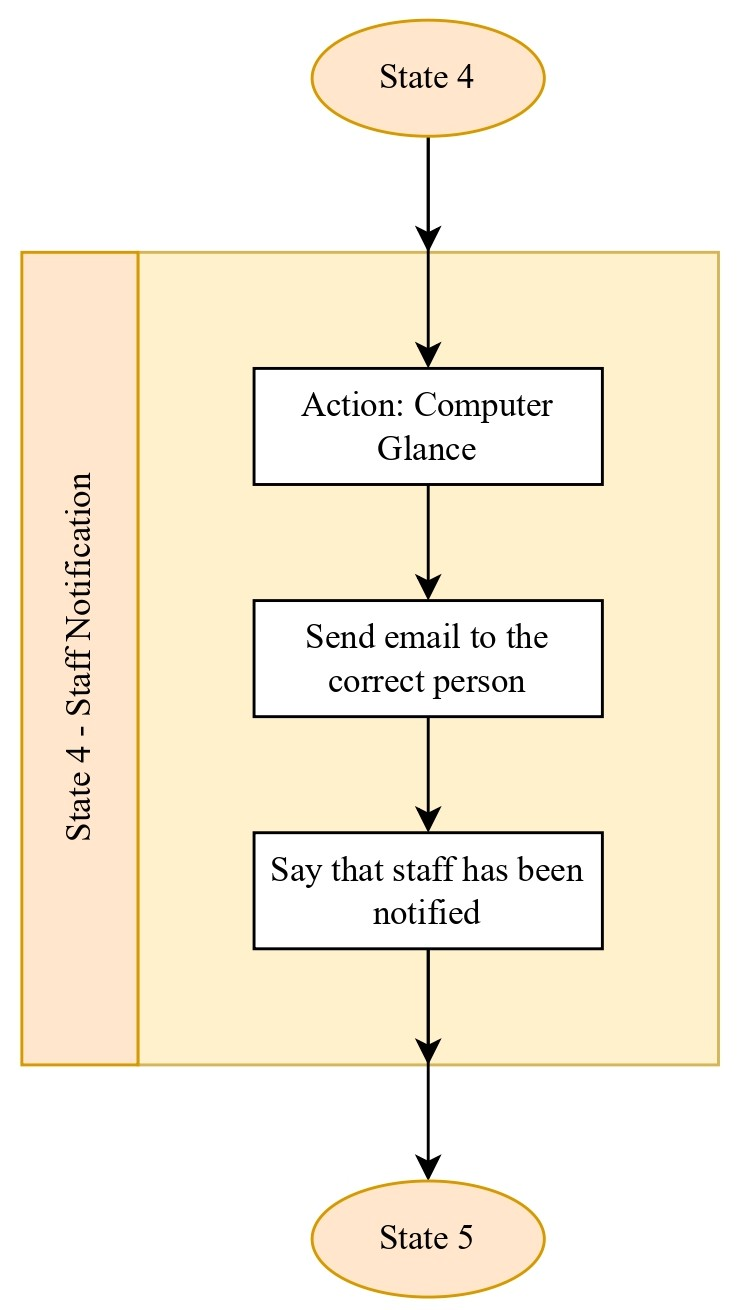
\includegraphics[width=.6\linewidth]{State 4 - Staff Notification.jpg}
    \caption{State 4 - Staff Notification}
    \label{State 4 - Staff Notification}
\end{figure}

\subsubsection{State 5}
\paragraph{Entry Condition:}
\mbox{}\\
Staff have been notified that a visitor is waiting.

\paragraph{Actions:}
\begin{itemize}
  \item Informs the user that staff will arrive soon.
  \item Asks the user to rate their experience, capturing input via \emph{Speech Recognition}.
  \item Runs \emph{Sentiment Analysis} to interpret the feedback.
  \item Thanks the user for their feedback.
  \item Monitors for any change in faces to detect if staff has arrived.
\end{itemize}

\paragraph{Transitions:}
\begin{itemize}
  \item If the staff’s face is now recognized, the system \emph{waves} and returns to \textbf{State 0}, ready for the next interaction cycle.
\end{itemize}

\begin{figure}
    \centering
    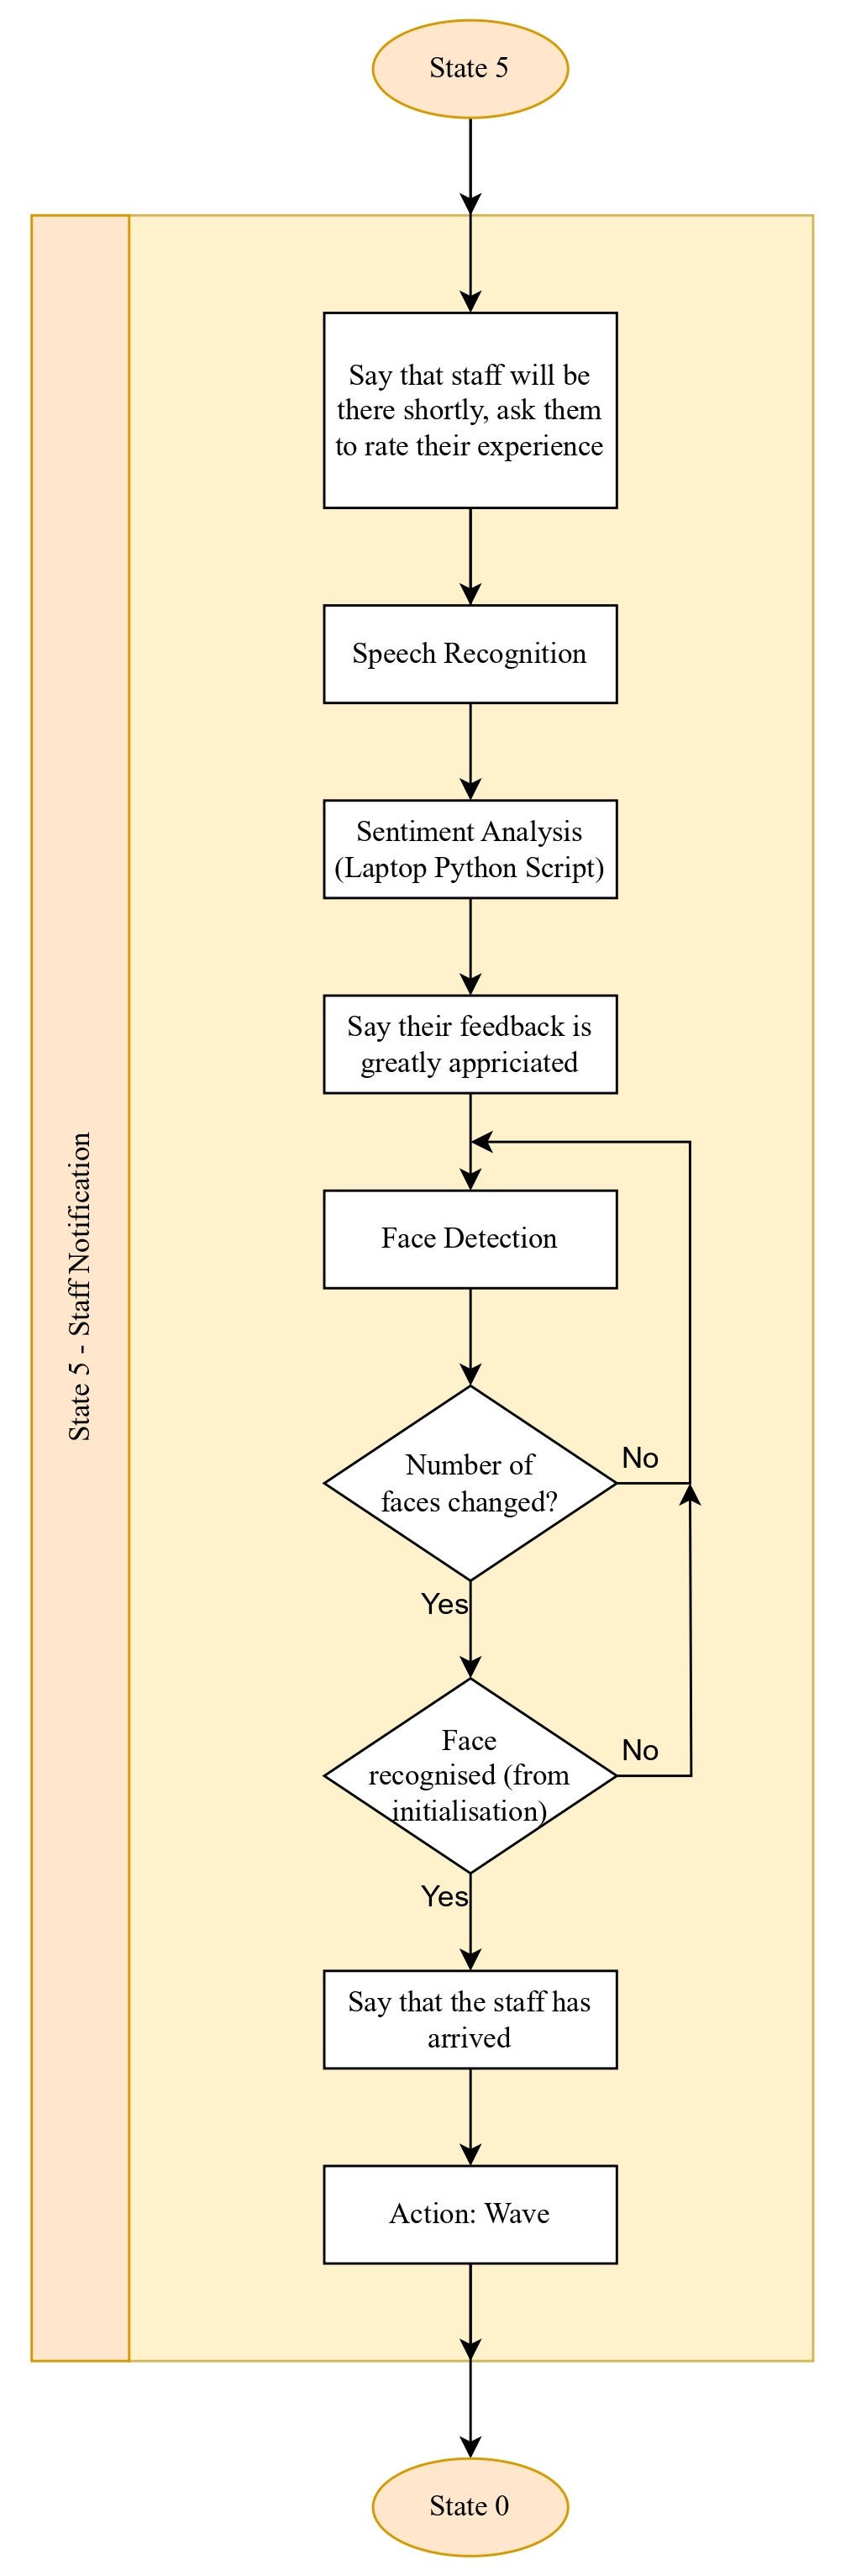
\includegraphics[width=.6\linewidth]{State 5 - Staff Notification.jpg}
    \caption{State 5 - Staff Notification}
    \label{State 5 - Staff Notification}
\end{figure}


\subsection{Sentences Spoken by the Robot}

The robot has several states (\textbf{State 0} to \textbf{State 5}), each with characteristic announcements or prompts. Below are samples of the main utterances (also visible in the previous subsection):

\begin{itemize}
  \item \textbf{State 1}:
    \begin{itemize}
      \item \texttt{``Hi, my name is Gordon, do you have an appointment?''} \\
    \end{itemize}

  \item \textbf{State 2}:
    \begin{itemize}
      \item \texttt{``Who do you have an appointment with?''} \\
            Prompts for the staff member’s name.
      \item \texttt{``May I ask for your confirmation number?''}
      \item \texttt{``Sorry, didn't catch that''} \\
            If speech recognition is unclear or fails.
      \item \texttt{``I've got you''} \\
            If a matching name/number was found.
      \item \texttt{``That is not in our database''} \\
            If no match is found for either the name or number.
    \end{itemize}

  \item \textbf{State 3}:
    \begin{itemize}
      \item \texttt{``Do you want to call a human?''}
    \end{itemize}

  \item \textbf{State 4}:
    \begin{itemize}
      \item \texttt{``I have sent an email to the member of staff.''} \\
    \end{itemize}

  \item \textbf{State 5}:
    \begin{itemize}
      \item Additional prompts about staff arrival and requesting user feedback.
    \end{itemize}
\end{itemize}



\subsection{Code Overview}

The project employs external webcamera vision system for hand gesture detection (wave detection, rude gestures from angry customers), integrating OpenCV and MediaPipe.

\subsubsection{Main Components}
\begin{itemize}
  \item \textbf{SimpleServer Class:} 
    \begin{itemize}
      \item Handles TCP socket communication, accepting client connections and sending messages.
      \item Manages concurrency using threads and locks to ensure safe communication between the robot and external clients.
    \end{itemize}
  \item \textbf{\texttt{detectWave} Function:} 
    \begin{itemize}
      \item Utilises OpenCV to capture video frames and MediaPipe to process hand landmarks.
      \item Detects waving gestures and rude gestures based on the relative positions of hand landmarks.
      \item Sends corresponding signals (e.g., ``Wave'', ``Rude'') to the connected client (NAO) via the server.
    \end{itemize}
  \item \textbf{\texttt{handle\_client} Function:} 
    \begin{itemize}
      \item Receives text input from the client socket.
      \item Analyses the sentiment of the received text using NLTK's VADER SentimentIntensityAnalyzer.
      \item Sends back a sentiment response (Positive/Negative/Neutral) to the client.
    \end{itemize}
  \item \textbf{\texttt{image\_processing} Function:} 
    \begin{itemize}
      \item Preprocesses video frames by flipping and converting color spaces for MediaPipe processing.
    \end{itemize}
\end{itemize}

\subsubsection{Interaction Diagram}

\begin{figure}[!ht]
\centering
\resizebox{0.9\columnwidth}{!}{
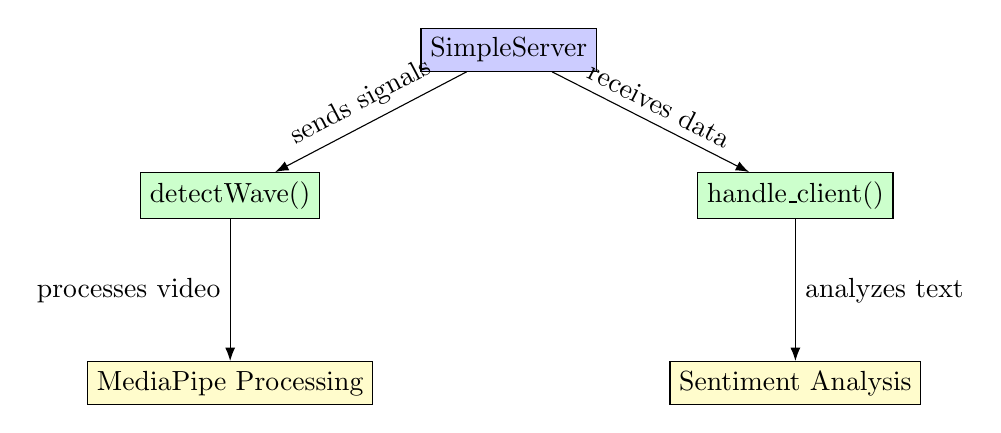
\begin{tikzpicture}[node distance=1.8cm, auto, >=Latex]
  % Nodes
  \node[rectangle, draw, fill=blue!20] (server) {SimpleServer};
  \node[rectangle, draw, fill=green!20, below left=of server] (detectWave) {detectWave()};
  \node[rectangle, draw, fill=green!20, below right=of server] (handleClient) {handle\_client()};
  \node[rectangle, draw, fill=yellow!20, below=of detectWave] (mediapipe) {MediaPipe Processing};
  \node[rectangle, draw, fill=yellow!20, below=of handleClient] (sentiment) {Sentiment Analysis};

  % Arrows
  \draw[->] (server) -- node[midway, above, sloped] {sends signals} (detectWave);
  \draw[->] (server) -- node[midway, above, sloped] {receives data} (handleClient);
  \draw[->] (detectWave) -- node[midway, left] {processes video} (mediapipe);
  \draw[->] (handleClient) -- node[midway, right] {analyzes text} (sentiment);
\end{tikzpicture}
}
\caption{System interaction flow diagram showing main components and their relationships}
\label{fig:interaction-diagram}
\end{figure}

\subsubsection{System Workflow}

\begin{enumerate}
  \item \textbf{Initialization:} The main program creates a \texttt{SimpleServer} instance, waiting for a client connection.
  \item \textbf{Wave Detection Loop:} Once connected, the system enters a loop calling \texttt{detectWave()}, processing camera frames to detect gestures.
  \item \textbf{Signal Communication:} Upon detecting a gesture, \texttt{detectWave()} spawns a thread to send the appropriate signal (e.g., "Wave", "Rude") via the server.
  \item \textbf{Client Handling:} Simultaneously, \texttt{handle\_client()} listens for incoming text data from the client, processes sentiment, and sends back a response.
\end{enumerate}

\subsection{GitHub} A shared GitHub housed README files, NAO scripts, and LaTeX documentation for report writing. Branches broke down project tasks and features, whilst version control assisted with project collaboration and testing. See Appendix for supporting GitHub documentation.

\subsection{Design Rationale} We opted for a height-aligned placement of NAO to improve authority and user engagement,
as recommended by Rae et al.\cite{Rae2013}. This also aligns with Sutherland et al.\cite{Sutherland2019}, who showed the benefits of
a robotic receptionist in clinical settings. This project expands on their Wizard-of-Oz study by allowing NAO to generate all behaviours without remote operators.

\subsection{Contingency Measures} In practice, user trust decreases sharply when robots show consistent errors, as reported by Bistolfi~\cite{Bistolfi2022}.
Therefore, clear fallback steps were embedded:
\begin{itemize}
        \item If the appointment check-in fails, staff are alerted via email.
\end{itemize}

\subsection{Hazard Mitigation} Following a risk assessment, a highlighted safety concern of NAO are the ‘pinch points’ during robotic movements. To avoid physical contact, NAO will be placed behind a desk and out of reach from the user.

\section{Testing and Results}

TBD

\section{HRI Dialogue Example}

\textit{[User wave detected]}
Gordon: Hi! My name is Gordon. Do you have an appointment?
User: Yes, I do.
Gordon: Who do you have an appointment with?
User: [unrecognisable mumbling]
Gordon: Sorry, didn't catch that.
User: I have an appointment with Bob.
\textit{[Gordon checks the database for an employee called Bob. Bob doesn’t exist.]}
Gordon: May I ask for your confirmation number?
User: My appointment number is 4.
\textit{[Gordon checks the database for a matching confirmation number. Confirmation number exists.]}
Gordon: I have got you.
\textit{[Gordon sends staff member an email]}
Gordon: I have sent an email to the member of staff. Someone will be with you shortly.  In the meantime, how would you rate your experience with me on a scale of 1 to 10?
User: 10! Your service was fantastic.
Gordon: Your feedback is greatly appreciated, thank you. 
\textit{[Gordon detects the staff member walking in]}
Gordon: Our staff is here to help you. Bye.

Scenario: A patient checks in with NAO. The user has an appointment with a staff member, however, that staff member does not exist, NAO prompts the user for their confirmation number. NAO locates the appointment and sends an email to the correct employee. Whilst the user is waiting, NAO asks for user feedback. NAO detects the staff member and announces their arrival.

This scripted scenario highlights two particular failure points anticipated in the system design. Firstly, NAO cannot recognise the user’s first response detailing who they have an appointment with. Secondly, the user mistakenly provides the name of someone who does not work there.  The system is designed to allow a maximum of two attempts to find the employee, then the user is prompted to provide a confirmation number. If the appointment is located, the script follows as above. Alternatively, if the appointment cannot be found, NAO can follow an expanded script asking if the user would like to speak with a human and emails the manager to assist. NAO can determine these failure points as the Python script contains a predetermined list of the employees. NAO listens for these predetermined words. If the user fails to correctly articulate an employee’s name from the predetermined list, NAO will then proceed with the contingencies put in place as part of the system design. To maintain a positive user experience, the user will only be prompted to repeat themselves once, beyond this, human intervention will be offered to avoid user frustrations with the robot. 


\section{Future Work}Facial recognition was planned and developed but was not able to be featured in the final testing due to 
technical difficulties. Future work on this project would include and expand upon this capability as recognising (and potentially 
analysing) individuals vastly increases the functionality and perceived intelligence of the system.

To improve the quality of the current conversations, integrating a more robust NLP algorithm increases the likelihood that the Nao 
robot correctly understands the user’s intent from a single output. Currently, any output outside of expected values is considered 
an error and handled accordingly. NLP allows more unexpected inputs to be parsed for key information that otherwise would’ve been 
missed, directing the robot towards a more appropriate response.

While these improvements would improve the technology, extensive user testing (especially within the intended medical space) is the 
best way to understand the system's shortcomings and improve accordingly.


\section{Discussion}
In general, HRI is an element that should be considered early in the design stage, allowing engineers to understand limitations of the system and manage user expectation.
\subsection{Plan vs implementation}
\textbf{Discuss how the final produced HRI solution differs from the initially presented state machine and dialogue. Include a discussion about the reasons for the differences.}

Compared to the initial design, there were a few parts added and some not included in the final solution produced. Added elements including gesture detection and NLP for a better user experience. Did not implement integration of NLP, external speech recognition for complex input, and creating face recognition library.

The gesture detection using opencv and mediapipe libraries to detect hand and landmarks, classifying the user's gesture. As co-speech gesture, it provides additional or reiterate information of the conversation to robot. In this application, wave detected indicates conversation starting or ending with users. Waving is an emblem gesture with a defined meaning of "Hello" or "Goodbye", that can help getting attention in human to human conversation, and usually the another person wave back. So it was decided that waving used as a key point of conversation starting in the robot and wave back as well. Making the interaction more realistic.

NLP includes test processing and nomization, tokenization, stemming, and lemmatization, part-of-speech tagging and syntactic parsing. It processes complicated text and get the abstract of idea. Such as analyzing sentiment of user feedback in this case. It was added to better understand complex input and extract useful information, and potential for further improvements based on the user feedback. NLP was implemented with Python code but not integrated with NAO. Because of the complex sentence, it was hard for NAO to recognize and transfer to text. That could be be improved in the future. Speech recognition for complex input was considered as a potential solution fitting with NLP but was not implemented because of the time limitation and subcription required for doing that.

Face recognition library was in the initial design, intended to learn different staff faces, then recognize and introduce them in front of the patient. It was not implemented in the final solution because of technical difficulty using the learn face and face recognize function from Choregraphe. Only one in ten attempts, learning and recognize face success. Different faces were tried and using the face detect first to only start learn or recognize face if there is one in front. Adding delay and loops for testing purpose also did not work. Would be a possible future improvement.


\subsection{Project Limitations}

\begin{enumerate} 
        \item \textbf{Limited speech recognition.} NAO’s speech recognition can struggle with diverse accents and dialects, and recognizing long and complex sentence. Integrating more advanced speech recognition software such as Microsoft Azure or Google Speech-to-Text can improve this with better accuracy. Moreover, NLP from nltk library such as tokenize can be used to understand complex input. Openai can be used to analysis input and improve NAO response to be more intelligent.
        \item \textbf{Restricted physical interaction.} NAO’s limited mobility may offer unrealistic or unidentifiable gestures to its users. To avoid confusions, NAO should maintain basic gestures, and, if required, a video feed on a tablet could supplement NAO’s intentions.
        \item \textbf{Accessibility issues.} Medical environments are subject to users with a diverse range of accessibility needs. The NAO robot required a user to see a sign, prompting the user to wave and initiate communication with the robot. If a user has sight impairments, NAO would not successfully check-in the user.  Advanced image recognition could be used to detect visual aids such as guide dogs or mobility canes. Upon detection, NAO could automatically be triggered into state 2, proceeding with checking-in. To build upon the robust nature of NAO in an environment with accessibility needs, a mitigation plan for each ailment could be developed along with supporting improvements to assist these users.
        \item \textbf{User acceptance and usability.} Older users may be uncomfortable interacting with robots and may find NAO confusing or intimidating. Providing visible instructions and support materials such as posters could encourage familiarity and engagement. Can be improved by doing system test with user like using coded prototype and doing interviews to collect feedback.
        \item \textbf{Unstable face recognition.} The face learning function which creates the library and recognition of face from the library were unstable. Using external camera like on laptop, and use other algorithm like YOLO for live video face detection and recognition can improve performance. Providing more stable face recognition on identifying staff. 
\end{enumerate}


\subsection{Module Feedback} The HRI module was both interesting and highly engaging. It achieved an excellent balance between critical theoretical knowledge on HRI system architectures and practical application using the NAO robot. The module’s emphasis on user-centred design and enhancing the overall user experience is an important skill to create successful projects.

A standout highlight was the BRL visit, which offered invaluable exposure to real-world applications of HRI technologies and reinforced the theoretical concepts covered in the module.

One potential improvement would be to increase contact time with the NAO robot, either through a loan system or extended lab sessions. This would allow students to spend more time experimenting with programming and troubleshooting fostering deeper learning and confidence for the assessment.



\section{Conclusion}

TBD

\bibliographystyle{plain}
\bibliography{references}

\end{document}
